%%%%%%%%%%%%%%%%%%%%%%%%%%%%%%%%%%%%%%%%%%%
%%% DOCUMENT PREAMBLE %%%
\documentclass[12pt]{report}

%\usepackage{natbib}
\usepackage{subfigure}
\usepackage{amsmath,amssymb,array,biblatex,bm,caption,fancyhdr,float,graphicx,indentfirst,parskip,url,vmargin}
\usepackage{amsmath}
\graphicspath{{images/}}
\addbibresource{project.bib}
\captionsetup[figure]{labelsep=period}
\begin{document}
\setlength{\parindent}{1em}
\vspace*{0.25cm}
\hrulefill
\thispagestyle{empty}
\begin{center}
    \begin{large}
        \sc{UM--SJTU Joint Institute
        \vspace{0.3em}\\
        Numerical solution of the Laplace’s equation using the relaxation method
        \vspace{0.3em}\\
        VP260 Project
        \vspace{0.3em}\\}
    \end{large}
    \hrulefill
    \vspace*{5cm}\\
    \begin{large}
        \sc{Project Group 20}
    \end{large}
\end{center}
\vfill
\begin{large}
    \sc{Group Members:}
\end{large}
\begin{table}[h!]
    \flushleft
    \begin{tabular}{ll}
        Cai Yiteng \hspace*{3em}&518370910007\hspace*{3em}\\
        Fang Han \hspace*{3em}&518370910009\hspace*{3em}\\
        Jie Ao \hspace*{3em}&518021910413\hspace*{3em}\\
        Liu Yihua \hspace*{3em}&518021910998\hspace*{3em}\\
        \\
        Date: \today
    \end{tabular}
\end{table}

\textit{We state that each of us has contributed equally to this project.}\\

Signature:\underline{\makebox[25em]{                                         }}
\hfill
\clearpage
\renewcommand{\thesection}{\arabic{section}}
\section{Introduction}
\paragraph{}Based on the course studied before, only electric potential and electric field with known charge distribution is able to be solved. However, in most cases the potential is only known on the boundary of the region. The equipotential surface of conductor at electrostatic condition might be a similar situation, but it’s hard to figure out if the charge distributes ununiformly. 
\section{Theoretical Background}
\subsection{The Potential Field}
\paragraph{}Consider a region space that does not contain electric charge in its interior and is enclosed by one or more conductors maintained at fixed potentials. Then by applying Laplace’s equation
$$\nabla^2 V=0.$$
\paragraph{}With given boundary conditions, the potentials as a function of region space can be solved numerically with help of computer.
\paragraph{}The key of this project is: in a region there is no charge, the value of the electric potential at a given point equals to the average value of the potential at surrounding points. The formula is 
\begin{equation}
    E=-\nabla V.
\end{equation}
\paragraph{}To confine the situation, only x and y dimensions are related to the potential. Consider a point P (x,y,z) and a cubic Gaussian surface with side $2\Delta l$ centered on P. \begin{figure}[H]
    \centering
    \includegraphics[width=0.8\linewidth]{1.png}
    \caption{The cubical Gaussian surface}
    \label{fig:my_label}
\end{figure}
\paragraph{}since the box is small, then an approximation is that the flux through each surface equals to the normal component at center of each surface times the are $(2\Delta l)^2$. Then we can obtain that
\begin{equation}
\begin{split}
    \phi_{E}=E_{x}(x+\Delta l,y,z)(2\Delta l)^2+(-E_{x}(x-\Delta l,y,z))(2\Delta l)^2\\
    +E_{y}(x,y+\Delta l,z)(2\Delta l)^2+(-E_{y}(x,y-\Delta l,z))(2\Delta l)^2=0.
\end{split}
\end{equation}
\paragraph{}Based on (1) the electric-field components to the same approximation are expressed as:
\begin{equation}
    \begin{split}
        E_{x}(x+\Delta l,y,z)\approx -\frac{V(x+\Delta l,y)-V(x,y)}{\Delta l},\\
        E_{x}(x-\Delta l,y,z)\approx -\frac{V(x,y)-V(x-\Delta l,y)}{\Delta l},\\
        E_{y}(x,y+\Delta l,z)\approx -\frac{V(x,y+\Delta l)-V(x,y)}{\Delta l},\\
        E_{y}(x,y-\Delta l,z)\approx -\frac{V(x,y)-V(x,y-\Delta l)}{\Delta l}.
    \end{split}
\end{equation}
Substituting the four values into Eq. 2, we can finally calculate that
\begin{equation}
    V(x,y)=\frac{V(x+\Delta l,y)+V(x-\Delta l,y)+V(x,y+\Delta l)+V(x,y-\Delta l)}{4}
\end{equation}
\subsection{The Relaxation Method}
\paragraph{}For this project, our goal is to find the potential of all the interior points enclosed by a given boundary with known potential. 
\paragraph{}According to Eq. 4, we can calculate the potential at a specific point by taking the average value of the four point near it. But we can see that, even for the point close to the boundary, we can know part of the potential for the neighbouring points. We cannot calculate the potential of all the interior points directly by utilizing the method we mentioned above. Thus, we would like to introduce the relaxation method.
\begin{figure}[H]
    \centering
    \includegraphics[width=0.35\linewidth]{3.png}
    \caption{Boundary conditions}
    \label{fig:my_label}
\end{figure}
\paragraph{}For example, if we want to calculate the potential for the interior points enclosed by the given boundary in Figure 2, we can first make a rectangular grid of points inside the box, which is shown in Figure 3.  
\begin{figure}[H]
    \centering
    \includegraphics[width=0.5\linewidth]{4.png}
    \caption{Rectangular grid inside the box}
    \label{fig:my_label}
\end{figure}

The relaxation method can be described as following steps:
\begin{enumerate}
    \item Set the initial conditions: the side length of the box L, the distance between each grid $\Delta l$, the potential $V_{0}$ at the boundary points and the relative accuracy $\epsilon$ expected for our calculation.
    \item Arbitrarily set the initial potential for the interior point. In our calculation, we basically set the initial potential as $\frac{V_{0}}{2}$.
    \item Apply the results we get in Eq. 4 for each interior point, i.e.
    $$V(x,y)=\frac{V(x+\Delta l,y)+V(x-\Delta l,y)+V(x,y+\Delta l)+V(x,y-\Delta l)}{4}$$
    We can get a new matrix $V_{new}$ for the potential of the interior points.
    \item Calculate the value
    $$Acc=\left\vert\frac{V_{new}-V}{V}\right\vert.$$
    If $Acc\geq\epsilon$, repeat the step 3. Stop until $Acc<\epsilon$.
\end{enumerate}
After calculating all the potential, we can also calculate the electric field with the formula
\begin{equation}
\begin{split}
    E_{x}(x,y)\approx-\frac{V(x+\Delta l,y)-V(x-\Delta l,y)}{2\Delta l}\\
    E_{y}(x,y)\approx-\frac{V(x,y+\Delta l)-V(x,y-\Delta l)}{2\Delta l}
\end{split}
\end{equation}
\clearpage
\section{Detailed Calculation of the Potential Field}
\subsection{System A}
The boundary condition is shown in Figure 4, with $V_{0}=1V$
\begin{figure}[H]
    \centering
    \includegraphics[width=0.3\linewidth]{3.png}
    \caption{Boundary condition for the system A}
    \label{fig:my_label}
\end{figure}
Firstly, we set the length L to 50, the distance $\Delta l$ to 1, the expected accuracy to 0.0001. Then we got the three plot below by using the MATLAB. The detailed results of our data in the matrix form and the detailed MATLAB code can be seen in the appendix document for this project. 
\begin{figure}[H]
    \centering
    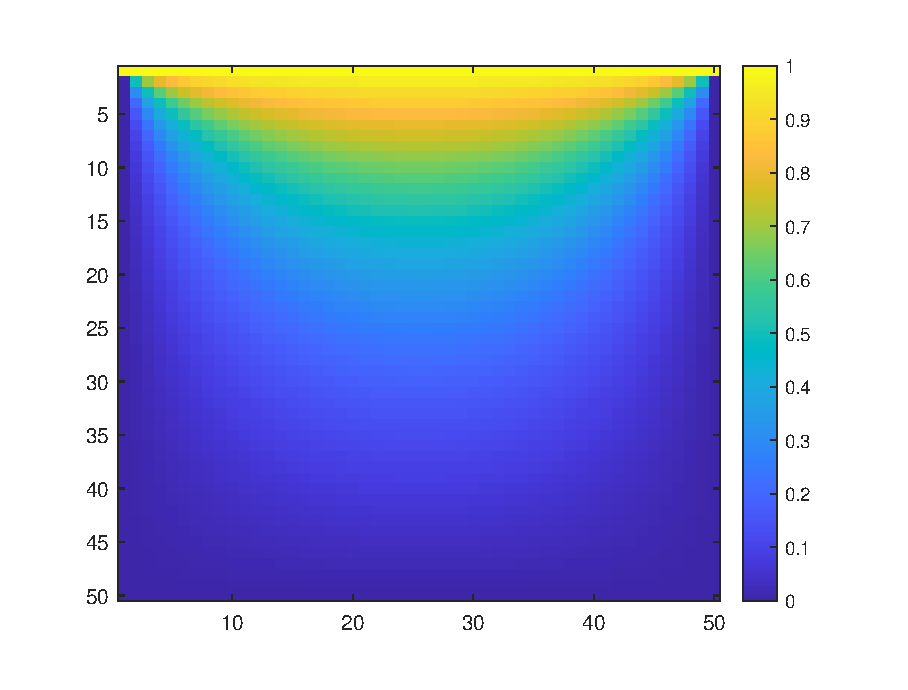
\includegraphics[width=0.8\linewidth]{A00001Density.eps}
    \caption{The density plot of the electrical potential of system A using 50*50 grid with accuracy 0.0001.}
\end{figure}
We can see that in Figure 5, the density of the electric potential gradually becomes sparse when the point comes close to the 0-potential boundary point.
\begin{figure}[H]
    \centering
    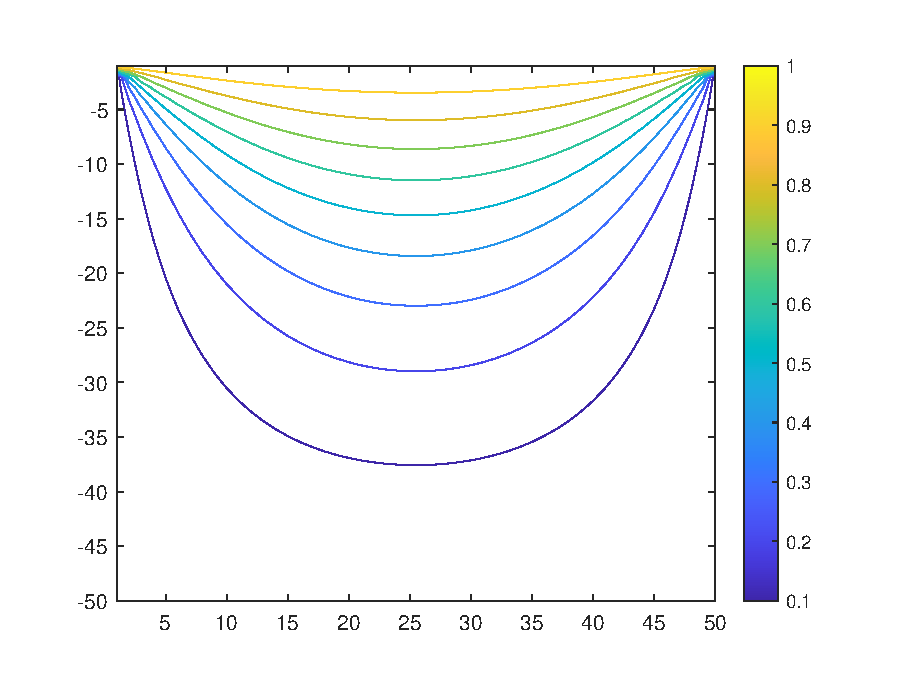
\includegraphics[width=0.8\linewidth]{A00001Contour.eps}
    \caption{The contour plot of the electrical potential (the equipotential lines) of system A using 50*50 grid with accuracy 0.0001.}
\end{figure}
\begin{figure}[H]
    \centering
    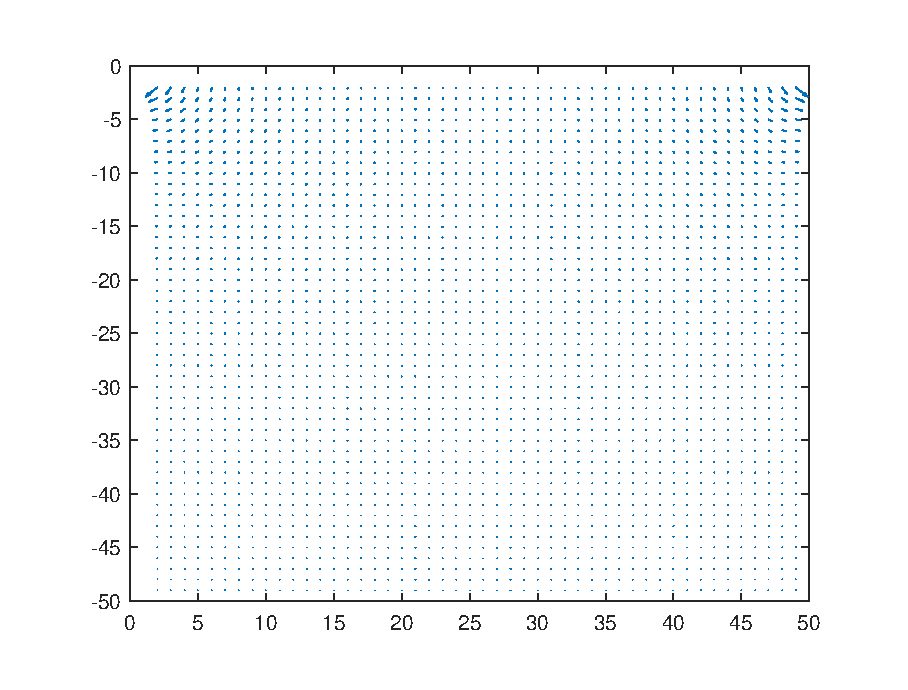
\includegraphics[width=0.8\linewidth]{A00001Vector.eps}
    \caption{The vector plot of the corresponding electric field of system A using 50*50 grid with accuracy 0.0001.}
\end{figure}
Then we plotted the graph with three different accuracy - 0.01, 0.001, 0.00001.
\begin{figure}[H]
    \centering
    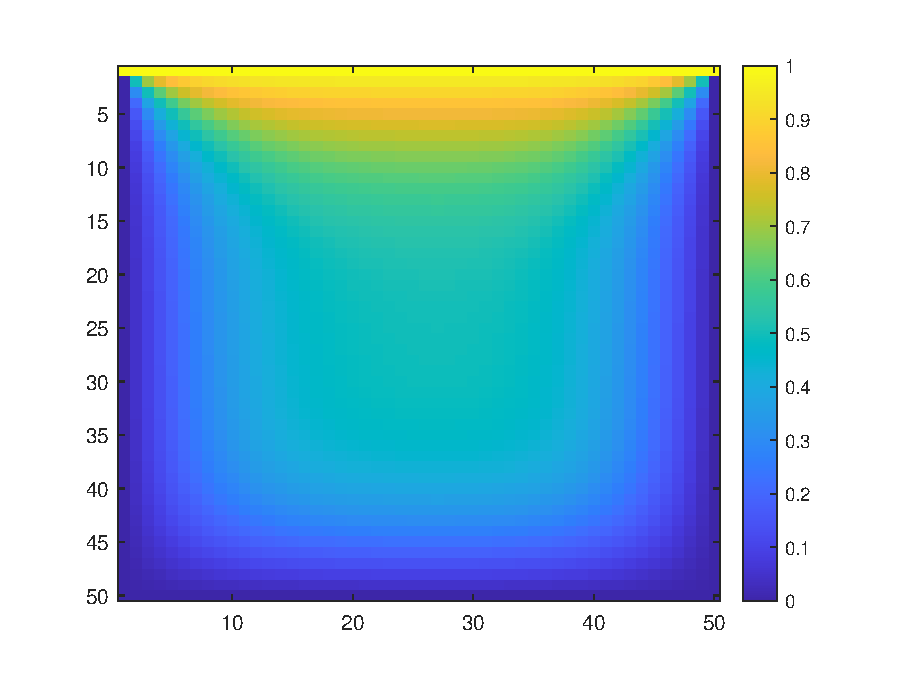
\includegraphics[width=0.8\linewidth]{A001Density.eps}
    \caption{The density plot of the electrical potential of system A using 50*50 grid with accuracy 0.01.}
\end{figure}
\begin{figure}[H]
    \centering
    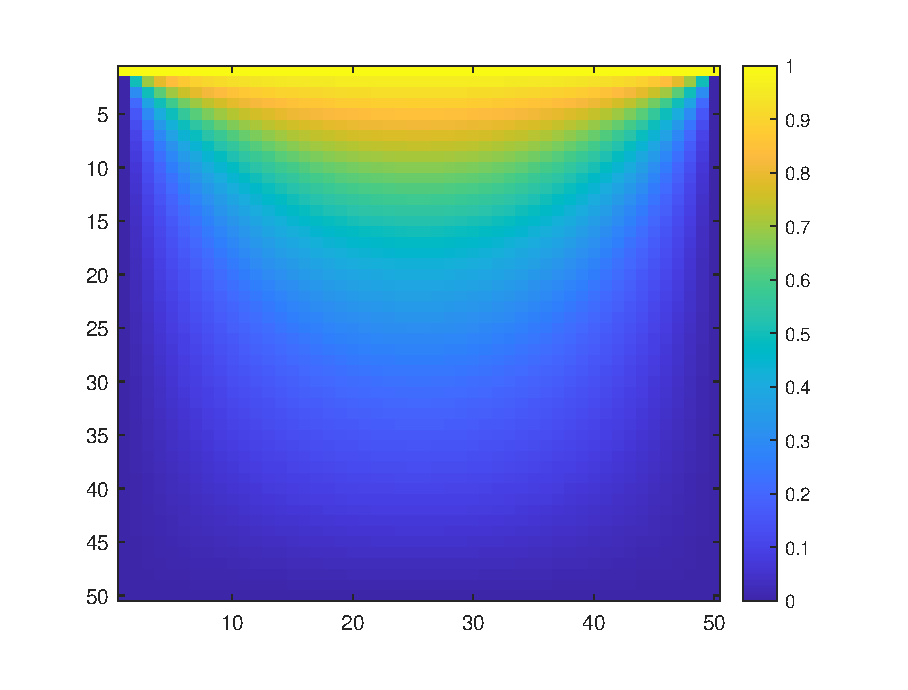
\includegraphics[width=0.8\linewidth]{A0001Density.eps}
    \caption{The density plot of the electrical potential of system A using 50*50 grid with accuracy 0.001.}
\end{figure}
\begin{figure}[H]
    \centering
    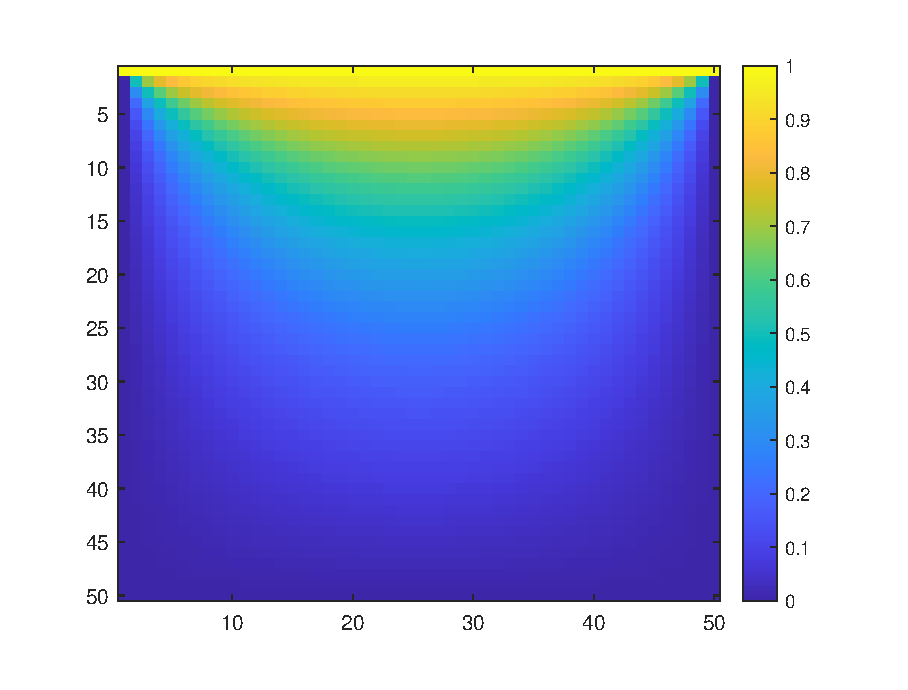
\includegraphics[width=0.8\linewidth]{A000001Density.eps}
    \caption{The density plot of the electrical potential of system A using 50*50 grid with accuracy 0.00001.}
\end{figure}
From Figure 8, Figure 9 and Figure 10, we can see that with the improvement of the accuracy, the transformation of the density becomes more smooth. This actually means our result come more close to the actual situation.
\begin{table}[H]
    \centering
    \begin{tabular}{|c|c|c|c|}
        \hline
        \multicolumn{2}{|c|}{Grid Size}&\multicolumn{2}{c|}{50}\\
        \hline
         Trial&Accuracy&Number of Iterations&Time Needed to Complete [s]\\
         \hline
        1 & 0.01 & 68 & 0.015448 \\
        \hline
        2 &0.001& 516 &  0.019710  \\
        \hline
        3 & 0.0001 & 1130  &  0.087856 \\
        \hline
        4 & 0.00001 & 1697 & 0.113464 \\
        \hline
    \end{tabular}
    \caption{Calculation data of system A.}
\end{table}
Still, setting the accuracy to 0.0001, we got the stage subplot in the density form and contour form by plotting the images of four different stages, i.e., the initial stage, the stage after 377 iterations, the stage after 753 iterations and the final stage.
\begin{figure}[H]
    \centering
    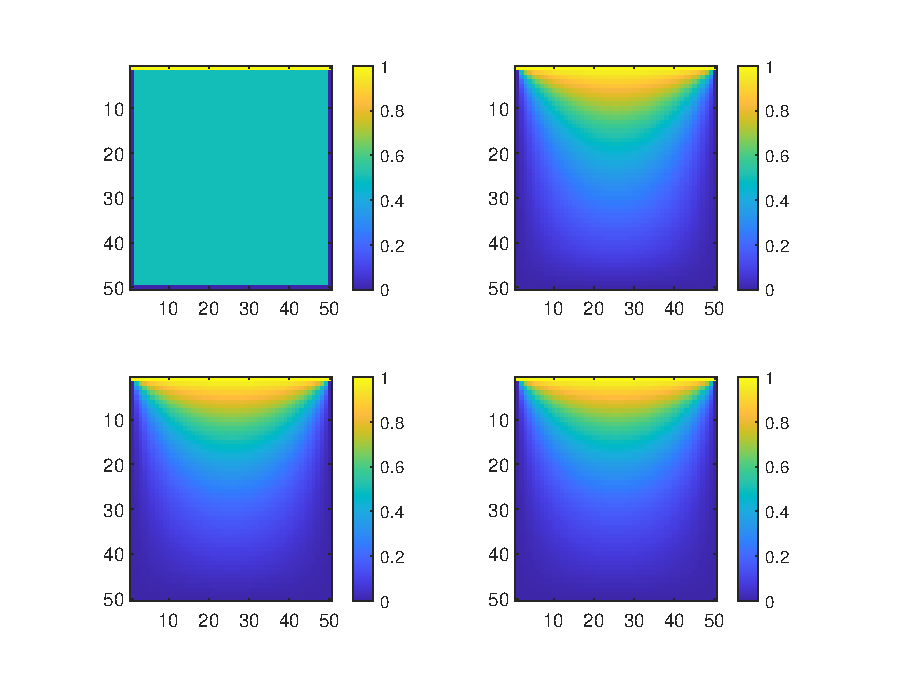
\includegraphics[width=0.8\linewidth]{AStageDensity.eps}
    \caption{The stage plot of the density of system A using 50*50 grid with accuracy 0.0001.}
\end{figure}
\begin{figure}[H]
    \centering
    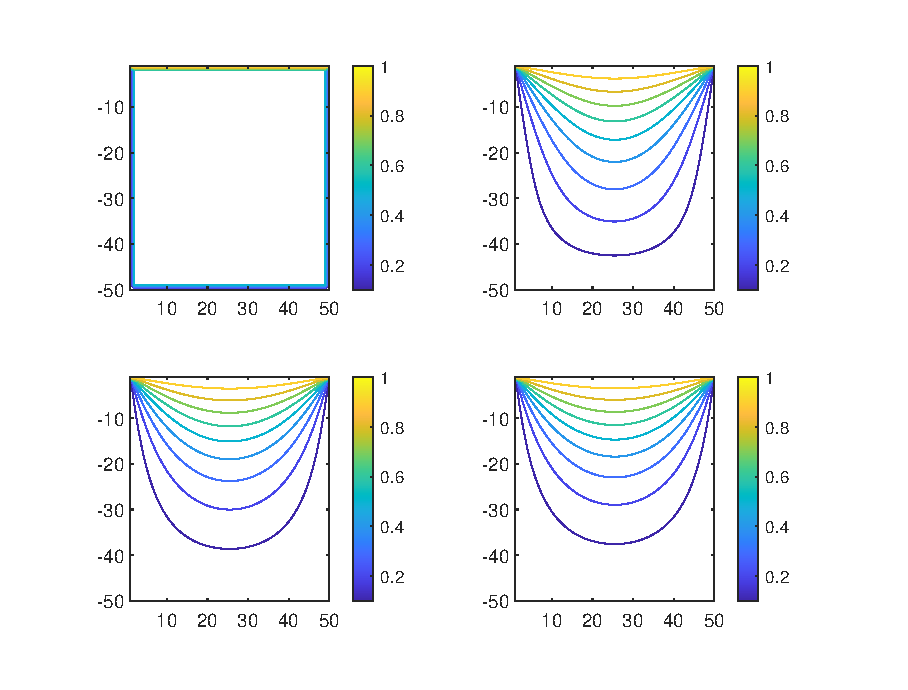
\includegraphics[width=0.8\linewidth]{AStageContour.eps}
    \caption{The stage plot of the contour of system A using 50*50 grid with accuracy 0.0001.}
\end{figure}
Similar to the situation when changing the accuracy, we can see that with the number of iterations increasing, the transformation of the density becomes more smooth. This is actually because of the two process are similar. If we expect the least accuracy, we will need to carry out fewer iterations.
\subsection{System B}
The boudary condition for the system B is basically the same as the system A. But the positive pole and the negative pole are exchanged and $V_{0}$ is still 1 V.

Firstly, we set the length L to 50, the distance $\Delta l$ to 1, the expected accuracy to 0.0001. Then we got the three plot below by using the MATLAB. The detailed results of our data in the matrix form and the detailed MATLAB code can be seen in the appendix document for this project. 
\begin{figure}[H]
    \centering
    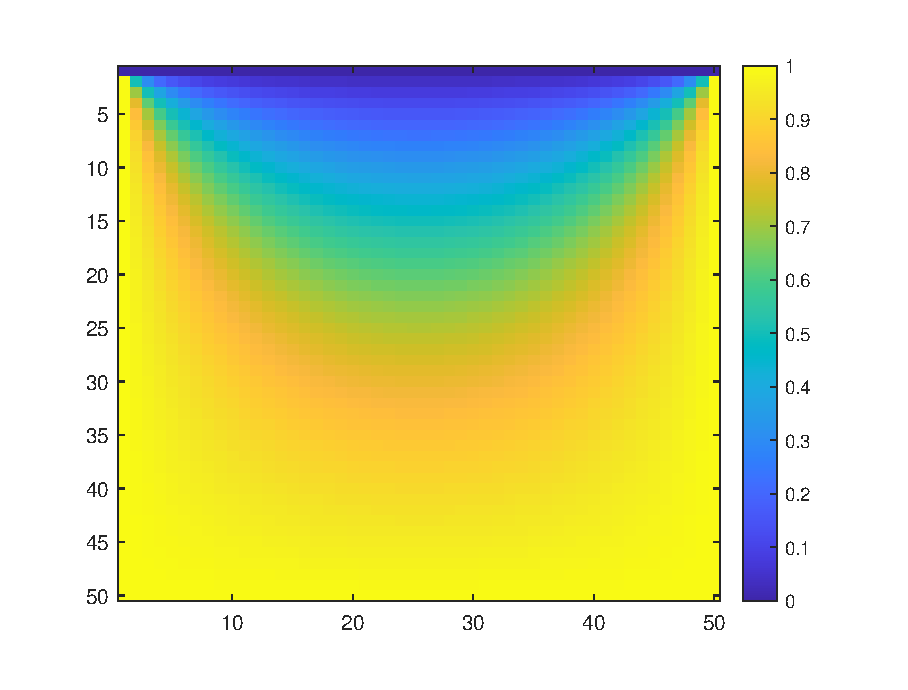
\includegraphics[width=0.8\linewidth]{B00001Density.eps}
    \caption{The density plot of the electrical potential of system B using 50*50 grid with accuracy 0.0001.}
\end{figure}
For the Figure 13, we can see that this figure has the similar form with Figure 5. This is because in the system B, we just changed the positive pole and negative pole. This means we just changed the magnitude of the density, but not the structure.
\begin{figure}[H]
    \centering
    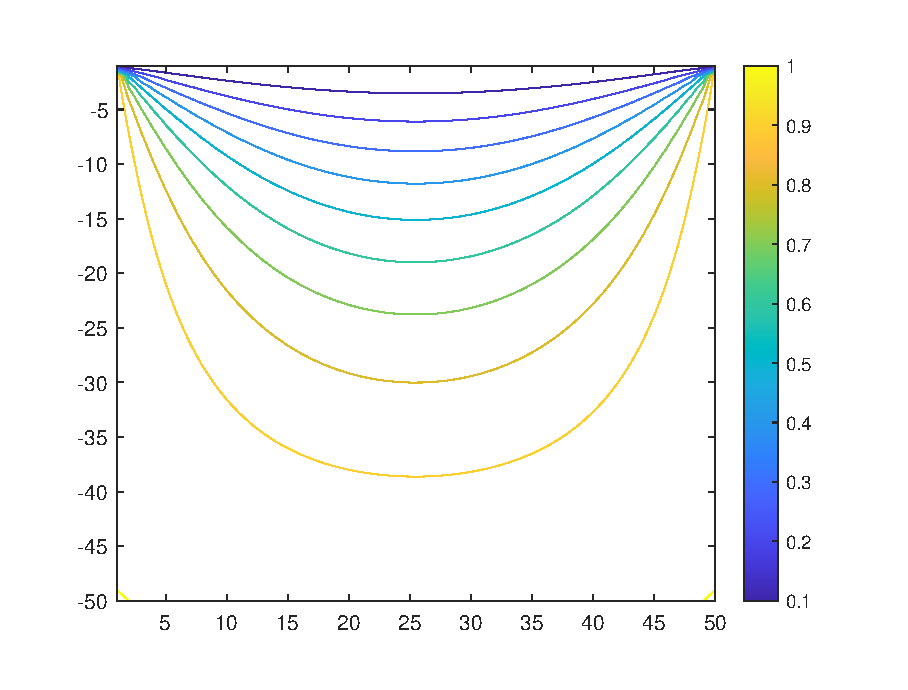
\includegraphics[width=0.8\linewidth]{B00001Contour.eps}
    \caption{The contour plot of the electrical potential (the equipotential lines) of system B using 50*50 grid with accuracy 0.0001.}
\end{figure}
\begin{figure}[H]
    \centering
    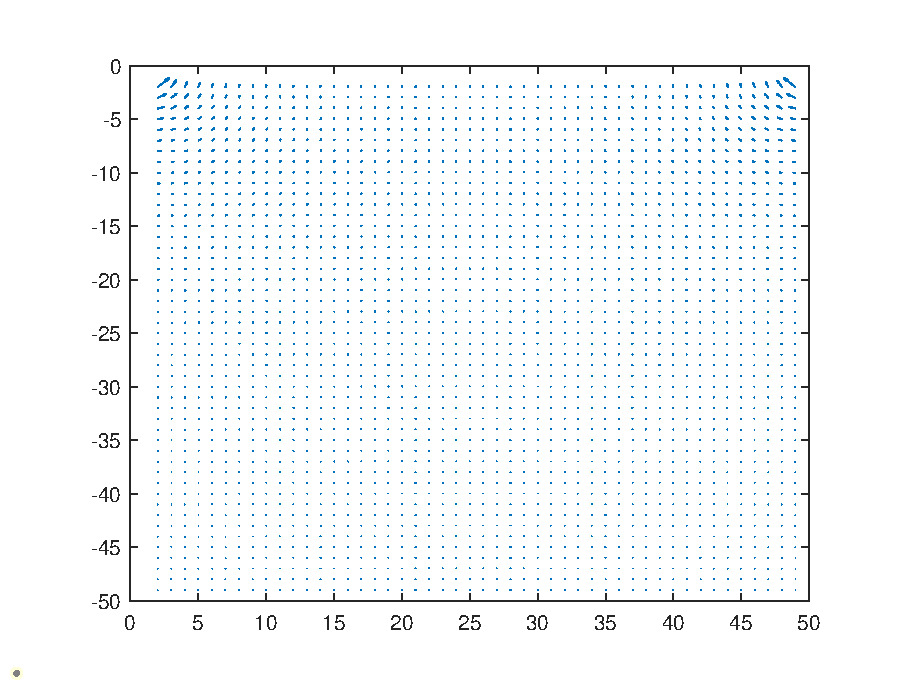
\includegraphics[width=0.8\linewidth]{B00001Vector.eps}
    \caption{The vector plot of the corresponding electric field of system B using 50*50 grid with accuracy 0.0001.}
\end{figure}
Also, we can see that Figure 14 and Figure 15 has the similar form with Figure 6 and Figure 7.

Then we plotted the graph with three different accuracy - 0.01, 0.001, 0.00001.
\begin{figure}[H]
    \centering
    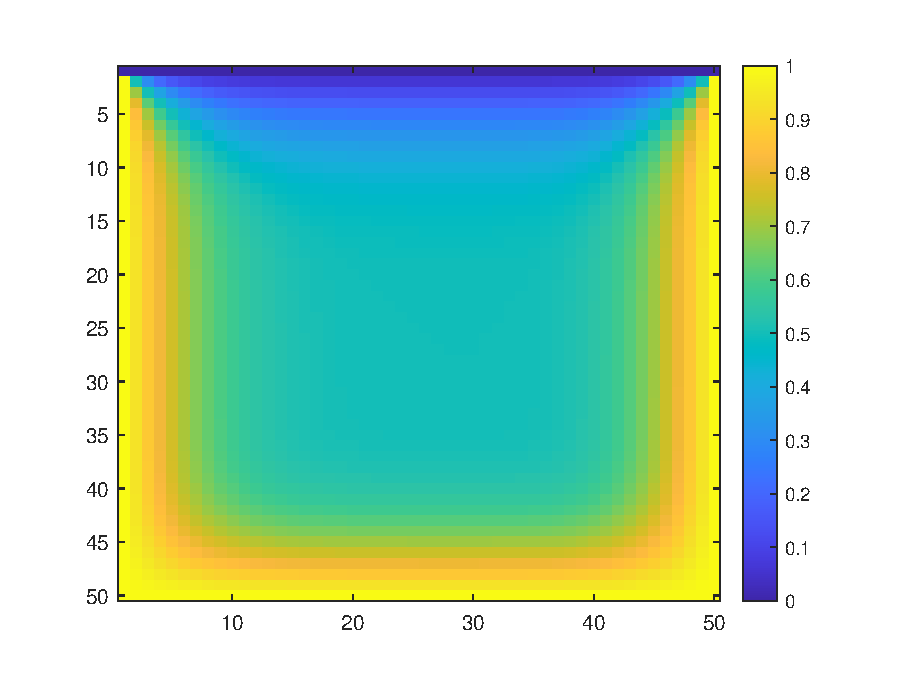
\includegraphics[width=0.8\linewidth]{B001Density.eps}
    \caption{The density plot of the electrical potential of system B using 50*50 grid with accuracy 0.01.}
\end{figure}
\begin{figure}[H]
    \centering
    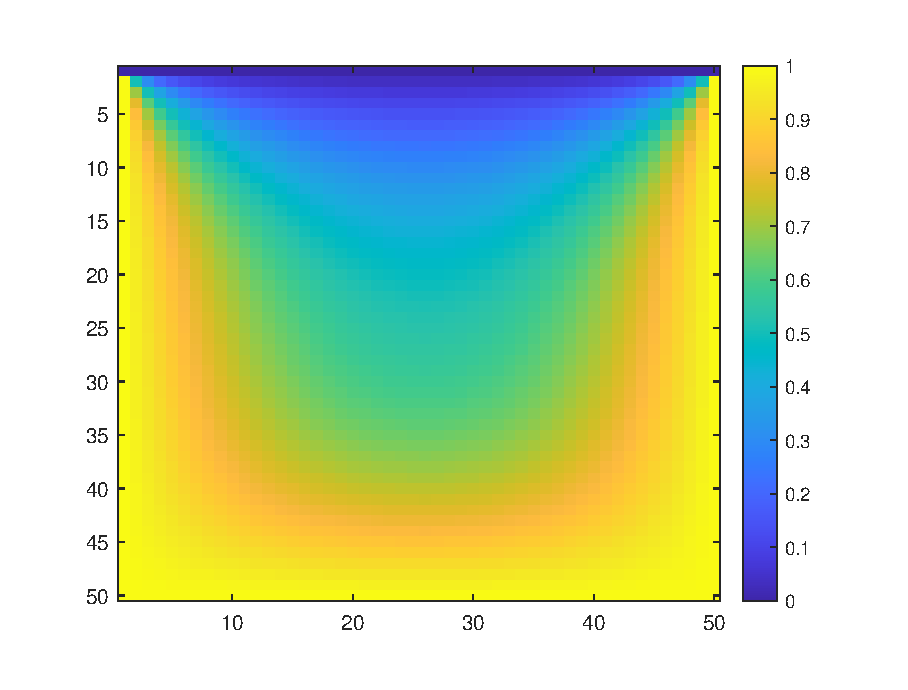
\includegraphics[width=0.8\linewidth]{B0001Density.eps}
    \caption{The density plot of the electrical potential of system B using 50*50 grid with accuracy 0.001.}
\end{figure}
\begin{figure}[H]
    \centering
    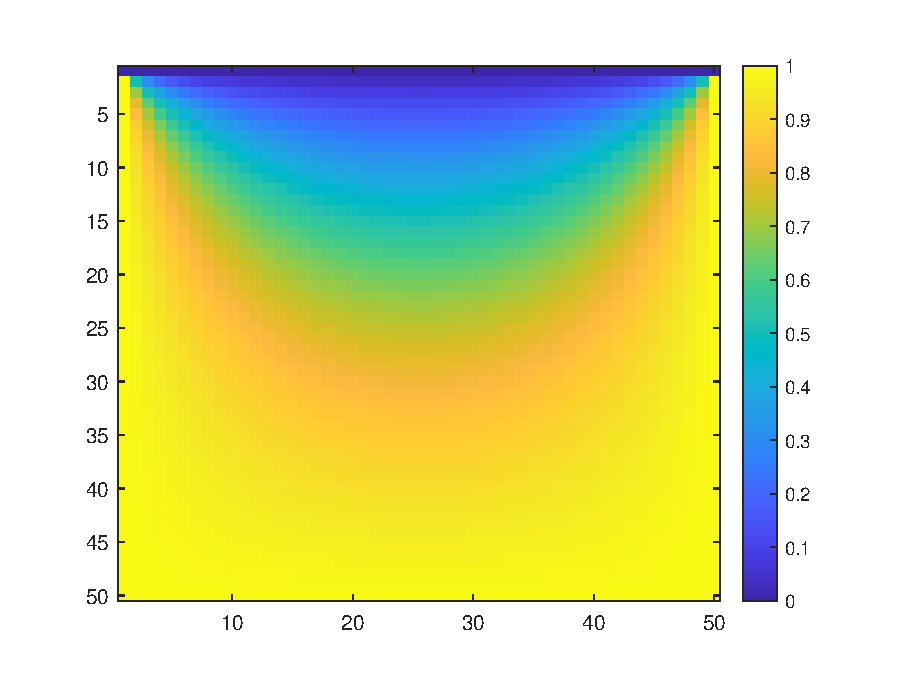
\includegraphics[width=0.8\linewidth]{B000001Density.eps}
    \caption{The density plot of the electrical potential of system B using 50*50 grid with accuracy 0.00001.}
\end{figure}

\begin{table}[H]
    \centering
    \begin{tabular}{|c|c|c|c|}
        \hline
        \multicolumn{2}{|c|}{Grid Size}&\multicolumn{2}{c|}{50}\\
        \hline
         Trial&Accuracy&Number of Iterations&Time Needed to Complete [s]\\
         \hline
        1 & 0.01 & 157 & 0.028861 \\
        \hline
        2 &0.001& 497 &  0.66686  \\
        \hline
        3 & 0.0001 &  1012 &  0.099173 \\
        \hline
        4 & 0.00001 & 1306 & 0.095325 \\
        \hline
    \end{tabular}
    \caption{Calculation data of system B.}
\end{table}
Still, setting the accuracy to 0.0001, we got the stage subplot in the density form and contour form by plotting the images of four different stages, i.e., the initial stage, the stage after 337 iterations, the stage after 675 iterations and the final stage.
\begin{figure}[H]
    \centering
    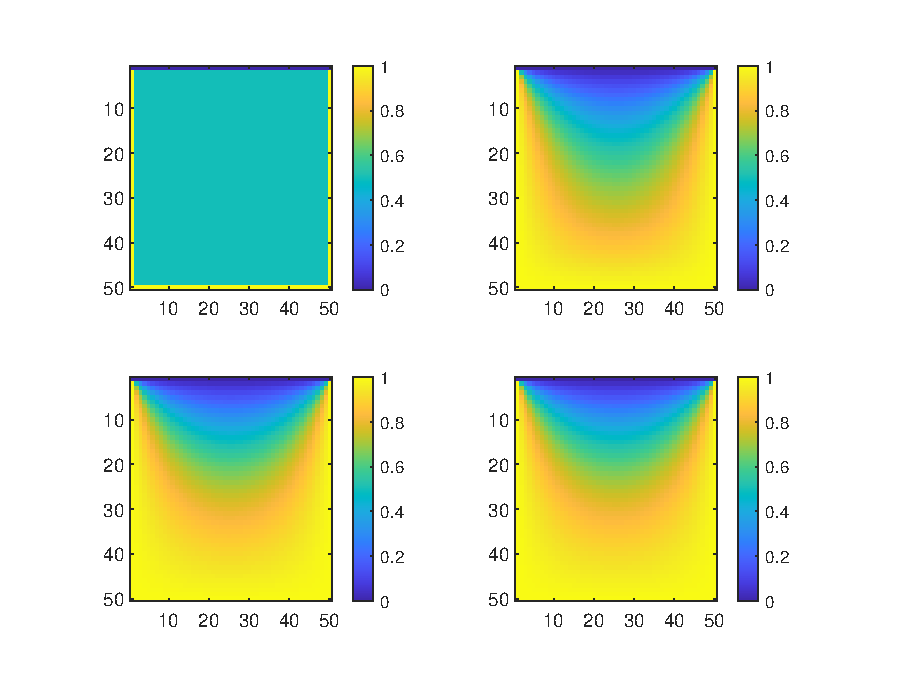
\includegraphics[width=0.8\linewidth]{BStageDensity.eps}
    \caption{The stage plot of the density of system A using 50*50 grid with accuracy 0.0001.}
\end{figure}
\begin{figure}[H]
    \centering
    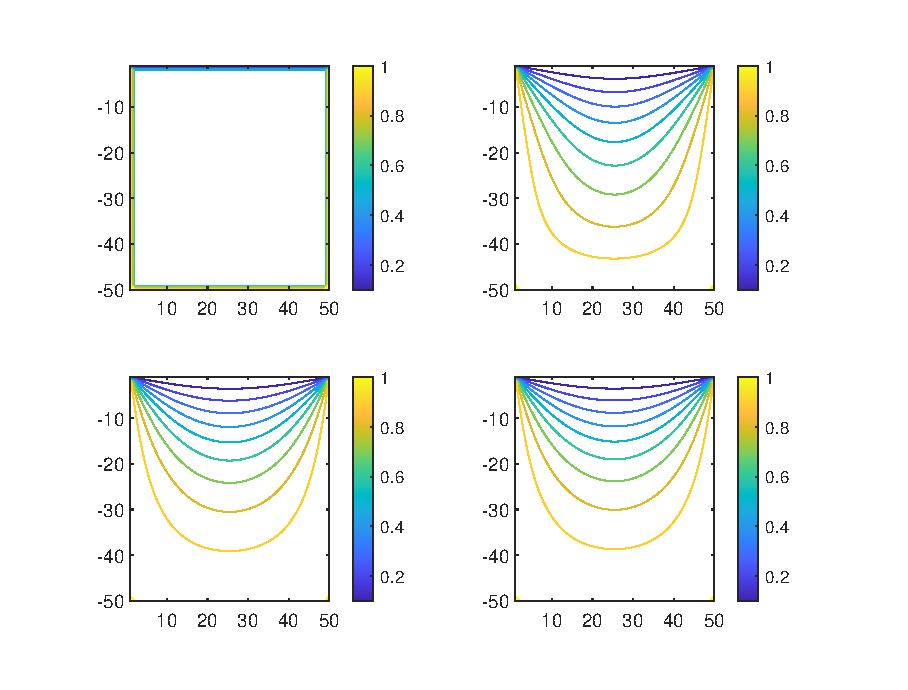
\includegraphics[width=0.8\linewidth]{BStageContour.eps}
    \caption{The stage plot of the contour of system A using 50*50 grid with accuracy 0.0001.}
\end{figure}
Actually, these results are similar to the form in system A.
\subsection{System C}
The boundary condition of the system C is shown in Figure 21, with $V0=1V$.
\begin{figure}[H]
    \centering
    \includegraphics[width=0.8\linewidth]{5.png}
    \caption{Boundary condition for the system C}
    \label{fig:my_label}
\end{figure}
Firstly, we set the length L to 50, the distance $\Delta l$ to 1, the expected accuracy to 0.0001. Then we got the three plot below by using the MATLAB. The detailed results of our data in the matrix form and the detailed MATLAB code can be seen in the appendix document for this project. 
\begin{figure}[H]
    \centering
    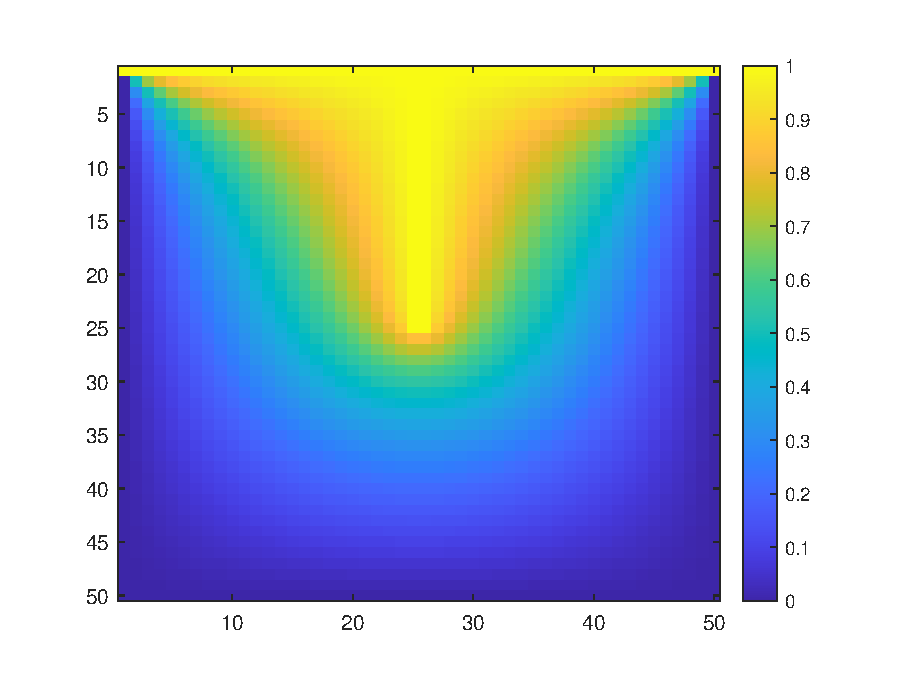
\includegraphics[width=0.8\linewidth]{C00001Density.eps}
    \caption{The density plot of the electrical potential of system C using 50*50 grid with accuracy 0.0001.}
\end{figure}
From Figure. 22, we can see that this figure differs from the two systems above since there is a 'finger' at the center of the box.
\begin{figure}[H]
    \centering
    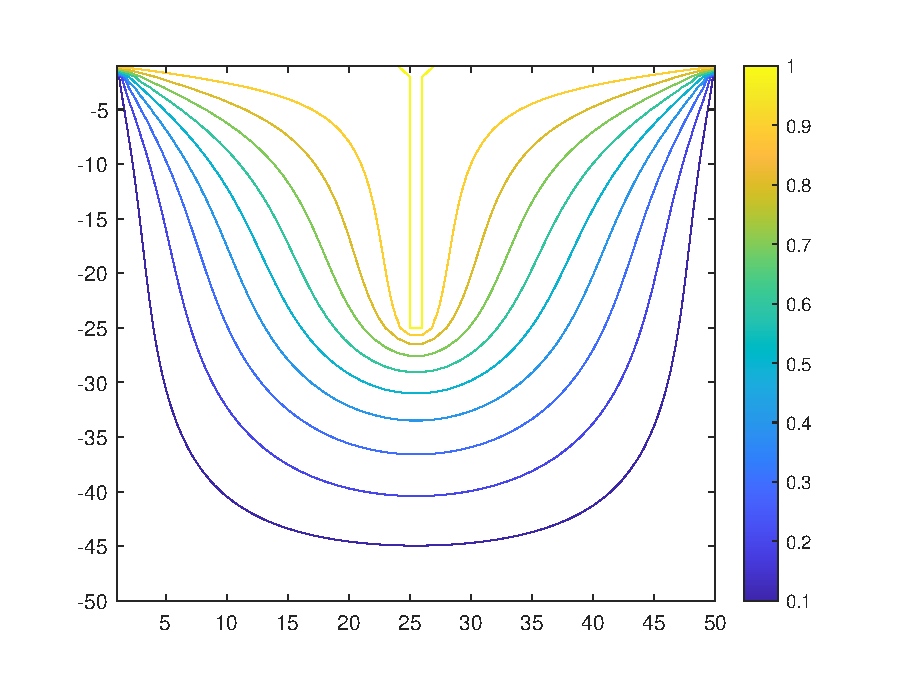
\includegraphics[width=0.8\linewidth]{C00001Contour.eps}
    \caption{The density plot of the electrical potential of system C using 50*50 grid with accuracy 0.0001.}
\end{figure}
\begin{figure}[H]
    \centering
    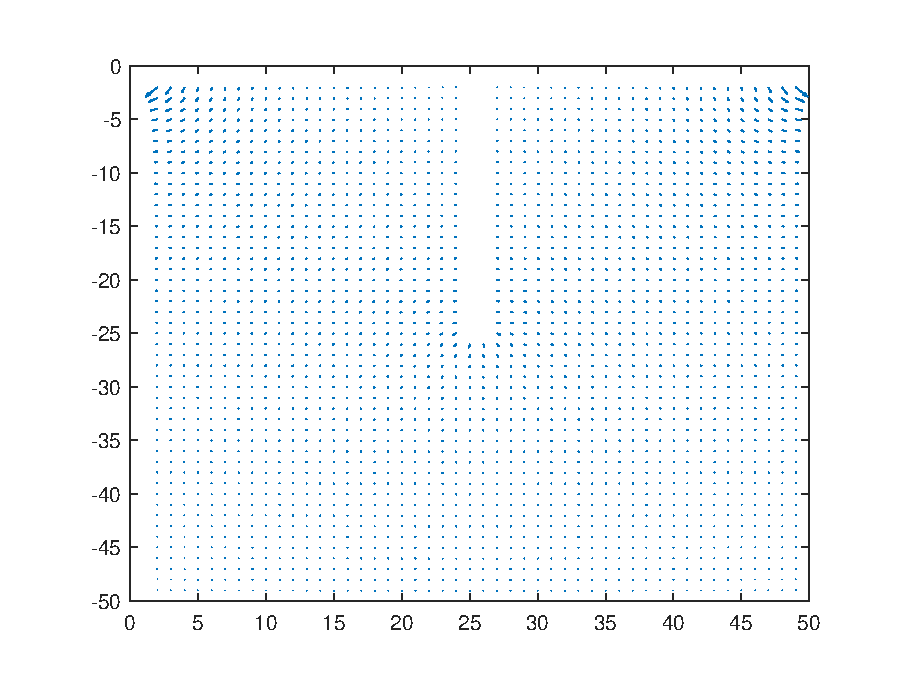
\includegraphics[width=0.8\linewidth]{C00001Vector.eps}
    \caption{The density plot of the electrical potential of system C using 50*50 grid with accuracy 0.0001.}
\end{figure}
Besides, from Figure 23 and Figure 24, we can see that the structure of the contour and the structure of the electric vector are also quite interesting. But they indeed correspond the theoretical model.
Then we plotted the graph with three different accuracy - 0.01, 0.001, 0.00001.
\begin{figure}[H]
    \centering
    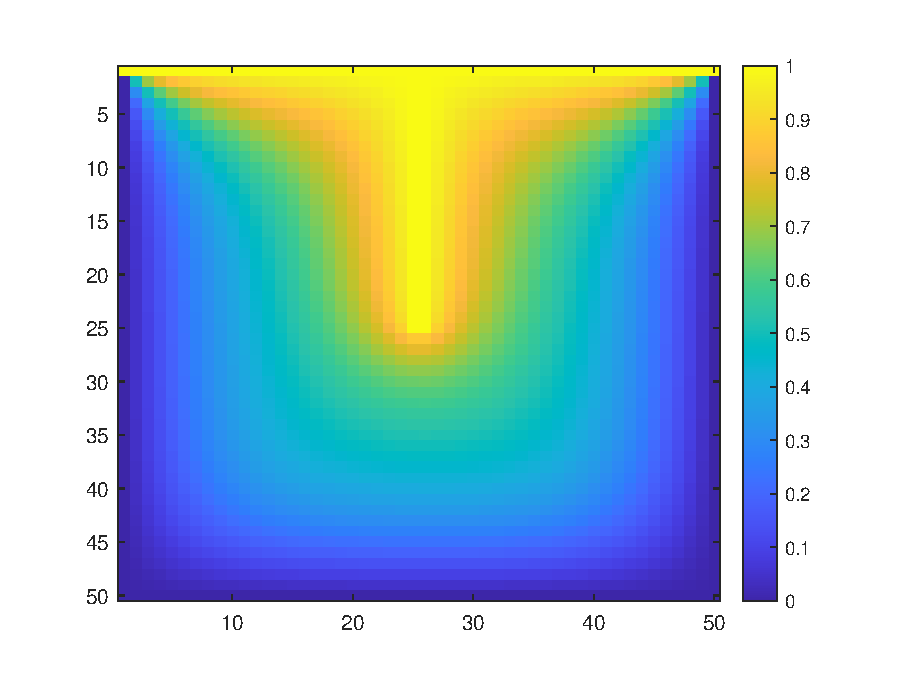
\includegraphics[width=0.8\linewidth]{C001Density.eps}
    \caption{The density plot of the electrical potential of system C using 50*50 grid with accuracy 0.01.}
\end{figure}
\begin{figure}[H]
    \centering
    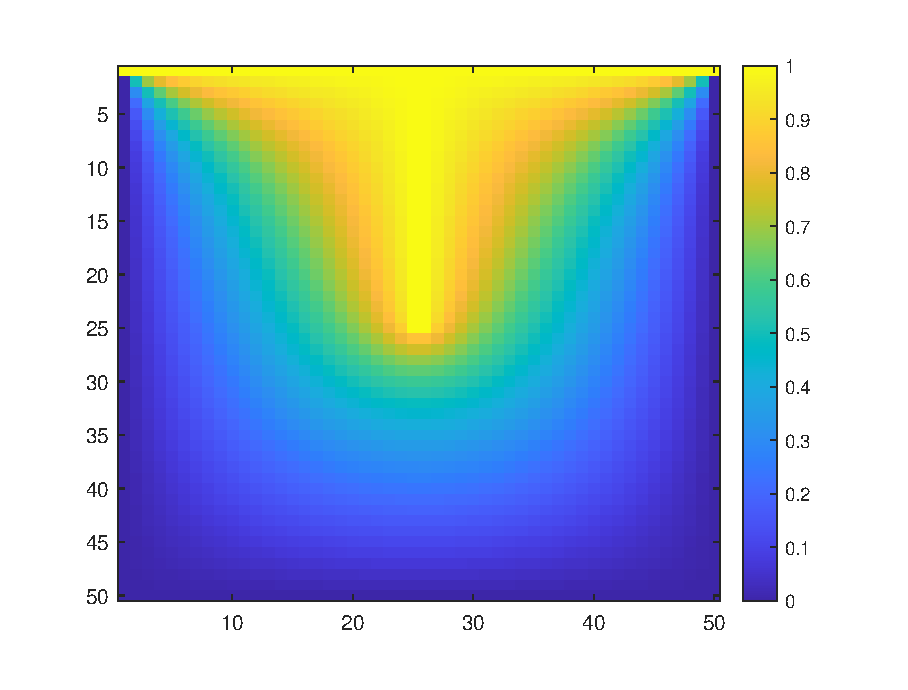
\includegraphics[width=0.8\linewidth]{C0001Density.eps}
    \caption{The contour plot of the electrical potential (the equipotential lines) of system C using 50*50 grid with accuracy 0.001.}
\end{figure}
\begin{figure}[H]
    \centering
    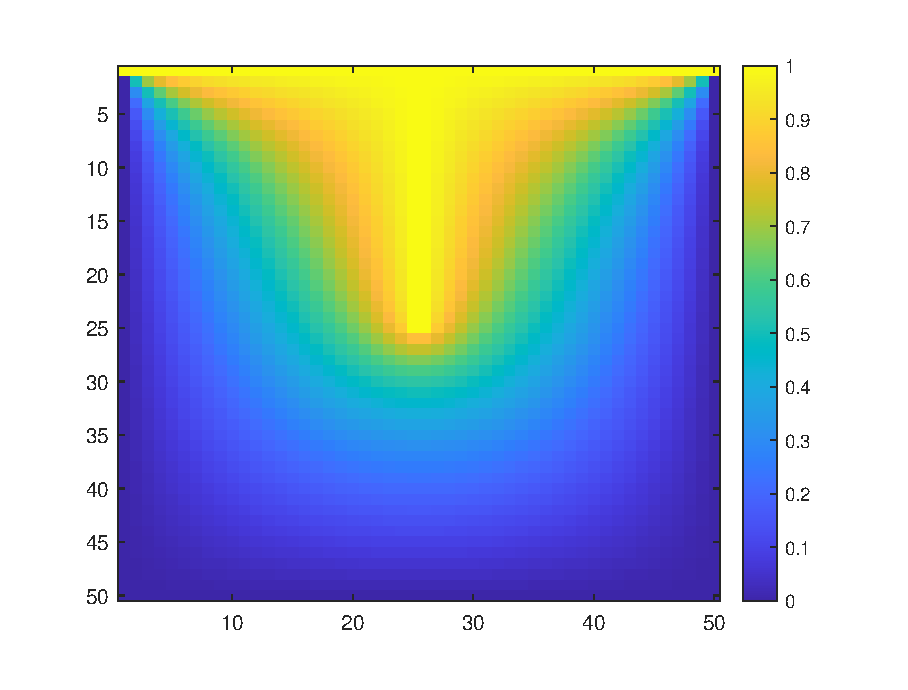
\includegraphics[width=0.8\linewidth]{C000001Density.eps}
    \caption{The vector plot of the corresponding electric field of system C using 50*50 grid with accuracy 0.00001.}
\end{figure}
From Figure 25, Figure 26 and Figure 27, we can also see the changes with the increase of the accuracy. The boundary becomes more smooth if we improve the accuracy.
\begin{table}[H]
    \centering
    \begin{tabular}{|c|c|c|c|}
        \hline
        \multicolumn{2}{|c|}{Grid Size}&\multicolumn{2}{c|}{50}\\
        \hline
         Trial&Accuracy&Number of Iterations&Time Needed to Complete [s]\\
         \hline
        1 & 0.01 & 68 & 0.025878 \\
        \hline
        2 &0.001& 305 &  0.064354  \\
        \hline
        3 & 0.0001 & 641  & 0.130604  \\
        \hline
        4 & 0.00001 & 967 & 0.215686 \\
        \hline
    \end{tabular}
    \caption{Calculation data of system C.}
\end{table}
Still, setting the accuracy to 0.0001, we got the stage subplot in the density form and contour form by plotting the images of four different stages, i.e., the initial stage, the stage after 214 iterations, the stage after 427 iterations and the final stage.
\begin{figure}[H]
    \centering
    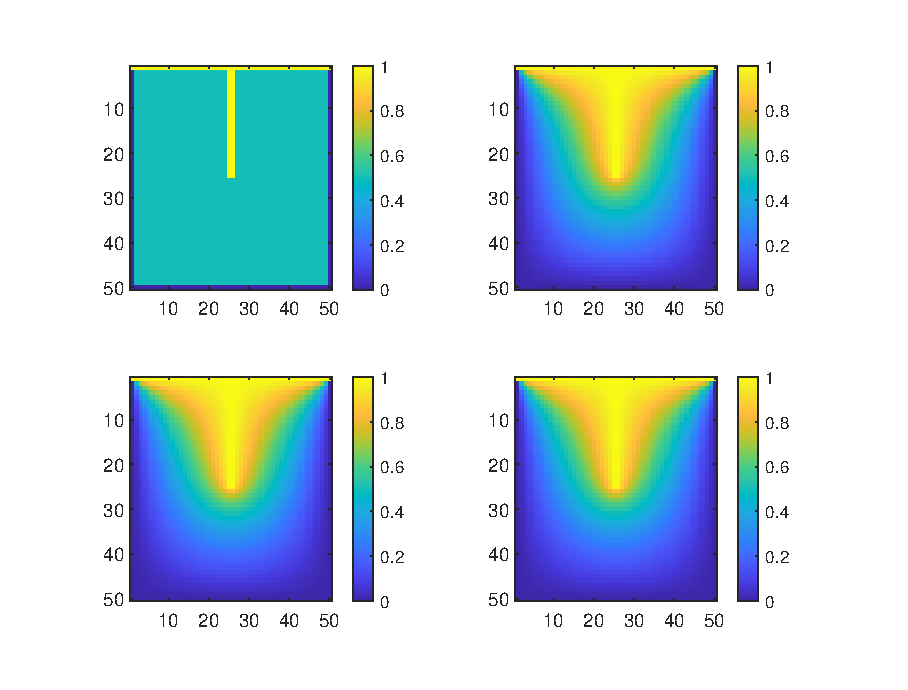
\includegraphics[width=0.8\linewidth]{CStageDensity.eps}
    \caption{The stage plot of the density of system C using 50*50 grid with accuracy 0.0001.}
\end{figure}
\begin{figure}[H]
    \centering
    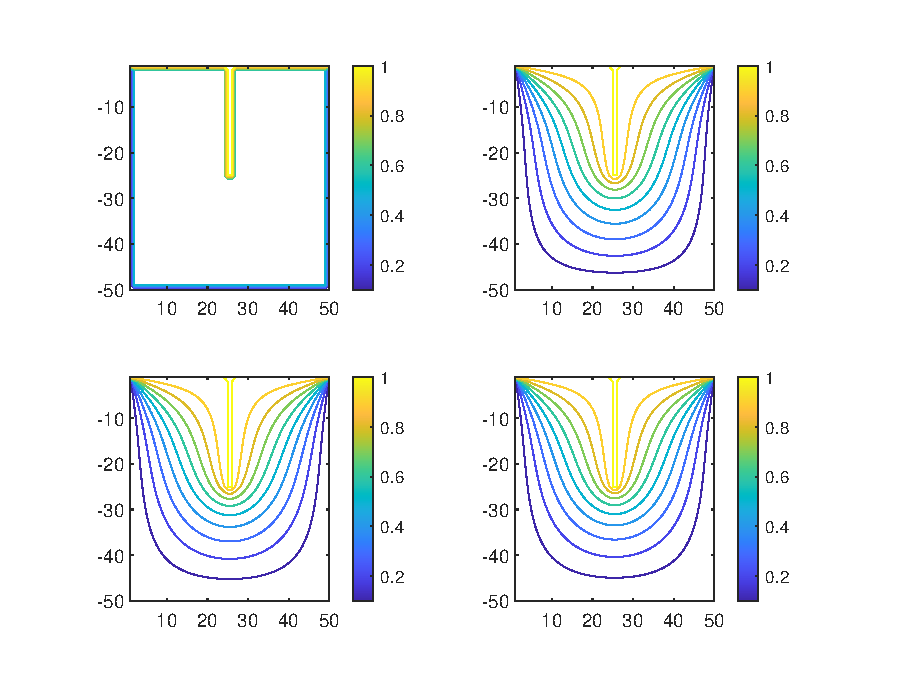
\includegraphics[width=0.8\linewidth]{CStageContour.eps}
    \caption{The stage plot of the contour of system C using 50*50 grid with accuracy 0.0001.}
\end{figure}
From Figure 28 and Figure 29, we can see that the stage plot clearly shows the variety from the initial stage to the final result, though the change in the last three figures is not so obvious.
\section{Conclusion and Discussion}
In this project, we investigated the numerical solution of the electric potential for the interior points with a known potential boundary. The relaxation method gave us a quite practical way to calculate the numerical value of some potentials. After calculating the detailed numerical results, we plotted the density of the electrical potential, the contour and the vector field of the electric field. This gives us a direct and vivid perspective of the electrical potential for the space we want to investigate. From these images, we can see that our calculate result actually follows the theoretical model.

However, for our calculations, there are several points to discuss: 
\begin{enumerate}
    \item In our calculations, we choose 50 for our side length. Actually, if we choose 100 for our side length, the transformation of the potential field will be more smooth than our results. However, if we set the side length to 100, our vector field will be too small for us to recognize. Thus, we finally choose 50 for our side length. 
    \item Besides, the stage form we choose may not be the best. Since in our calculations, our choice for each stage form is to just divide the total iterations by 3. This is actually not a best choice since in the first few iterations, the change of the electric potential will be the most obvious. Thus, if we want to see the uniform change of the electrical potential, we would better set another stage form. However, We have a fluent version of transformation in our appendix and this can better show the transformation in the process of the calculation.
\end{enumerate}
\clearpage
\section{Appendix}
In the appendix document, there are several things included:
\begin{enumerate}
    \item The numerical results of the calculation in the matrix form
    \item The MATLAB code for the system A, B and C
    \item The animated progress of the relaxation method, with the normal speed, the ten-times speed.
\end{enumerate}
The running time of our MATLAB code is measured by the computer equipped with Intel(R) Core(TM) i7-8750H CPU @ 2.20GHz.
\end{document}
